%##############################################%
% aspectosgerais < Desenvolvimento             %
% consideracoes < Metodologia                  %
% textoepostexto < Resultados                  %
% elementosdotexto < Conclusão                 %
%##############################################%


\chapter[Resultados]{Resultados}

	Através da verificação automática feita utilizando a ferramenta OpenSSL, em conjunto com \textit{scrypts}, foram alcançados resultados, vistos no gráfico~\ref{fig:graph01}. Esses resultados retornaram uma tabela, cujos valores incluem se as verificações encontraram algum erro e qual foi o erro encontrado, além de identificarem em quais certificados foram encontrados cada um dos erros.

	\begin{figure}[h]
		\centering
		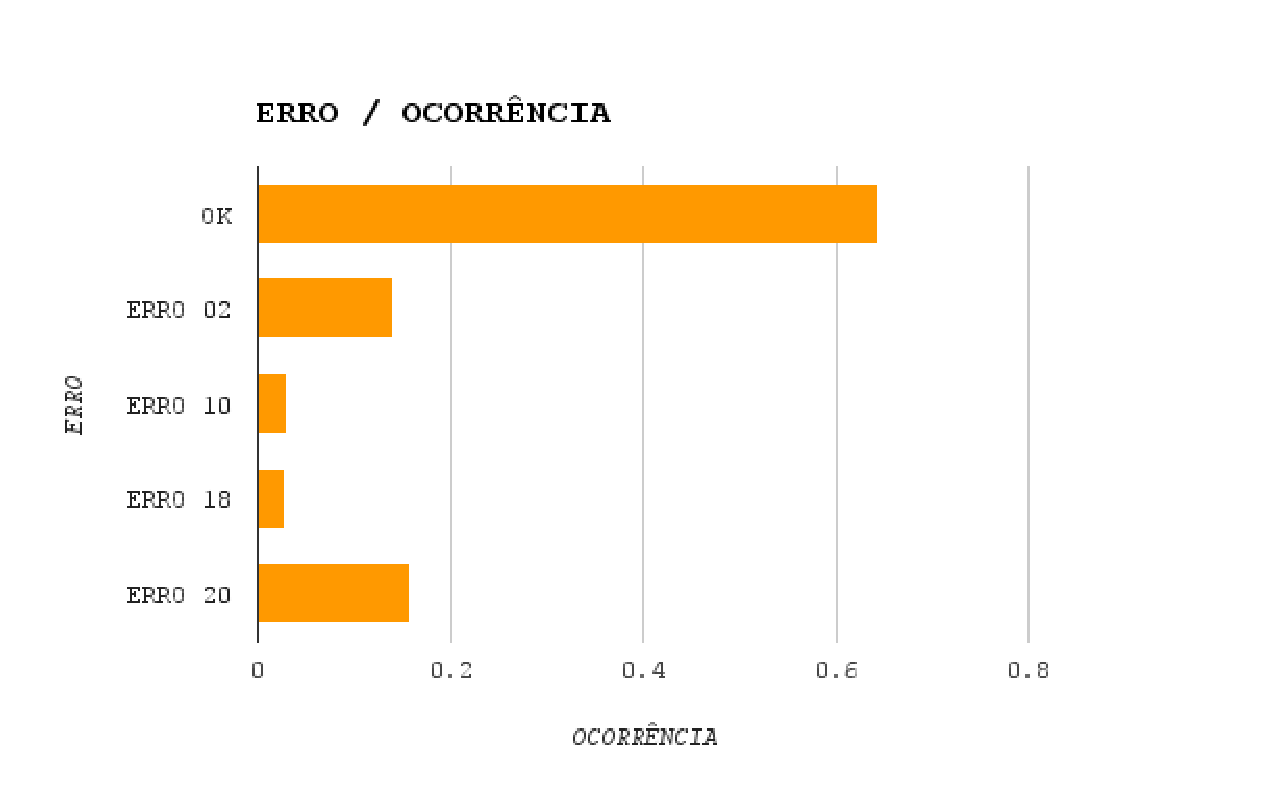
\includegraphics[keepaspectratio=true,scale=1]{figuras/graph01.eps}
		\caption{Taxa de Ocorrência dos Erros}
		\label{fig:graph01}
	\end{figure}

	Os números com que os erros se repetiram foram um dos dados extraídos da tabela, que se baseia na verificação de 799 (setecentos e noventa e nove) certificados digitais. Vale notar, também, que destes certificados verificados, foram considerados certificados de pessoa jurídica em sites de qualquer domínio.

	Os erros constatados são apresentados em proporção à suas ocorrências, como visto no gráfico~\ref{fig:graph02}.

	\begin{figure}[h]
		\centering
		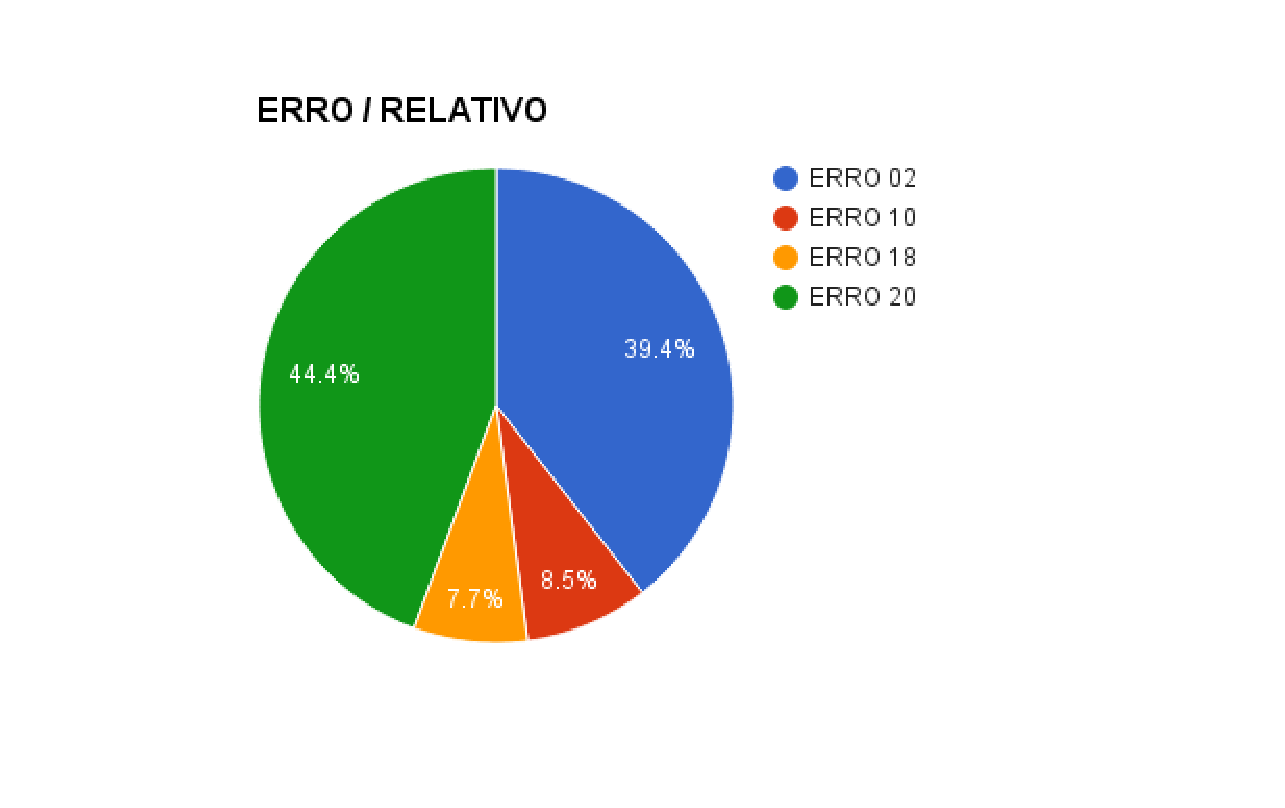
\includegraphics[keepaspectratio=true,scale=1]{figuras/erRel.eps}
		\caption{Taxa de Erros Relativos}
		\label{fig:graph02}
	\end{figure}

\section[Sem Erro]{Sem Erro}


	Os certificados que não apresentaram erros na verificação representam aproximadamente 64,45\% (sessenta e quatro por cento) dos certificados verificados no primeiro momento do trabalho. Esses certificados estão, de acordo com a verificação feita pela ferramenta OpenSSL, de acordo com as exigências dos PKCSs que adotam o padrão x509 como formato final.

\section[Erro 02 - Unable to get issuer Cetificate]{Erro 02 - Unable to get issuer Cetificate}

	Na documentação da ferramenta OpenSSL, o erro 02 (dois) identifica que a verificação retornou a mensagem: Incapaz de conseguir o certificado do emissor.
	Esse erro se apresenta quando a cadeia de certificados não está completa na listagem disponível no certificado analisado. O erro 02 (dois) se apresentou em aproximadamente 14\% (quatorze por cento) dos certificados verificados.

\section[Erro 10 - Certificate has Expired]{Erro 10 - Certificate has Expired}

	Na documentação da ferramenta OpenSSL, o erro 10 (dez) identifica que a verificação retornou a mensagem: O certificado expirou.
	Esse erro se apresenta se, e somente se, o certificado estiver sendo utilizado além de sua validade original. Um certificado digital tem um período de validade especificado no momento em que ele é emitido, e uma vez que esse prazo se cumpriu, ele deixa de ser reconhecido como válido. O erro 10 (dez) se apresentou em aproximadamente 3\% (três por cento) dos certificados verificados.

\section[Erro 18 - Self Signed Certificate]{Erro 18 - Self Signed Certificate}

	Na documentação da ferramenta OpenSSL, o erro 18 (dezoito) identifica que a verificação retornou a mensagem: Certificado auto-assinado.
	Neste caso em específico, duas condições foram encontradas irregulares no certificado. A primeira e mais evidente é que o alvo da certificação e o emissor do certificado são a mesma entidade; a segunda que se apresenta é que o certificado não se encontra na lista de certificados confiáveis, o que significa que ele não é uma autoridade certificadora raiz.
	O erro 18 (dezoito) se apresentou em aproximadamente 2,75\% (dois vírgula setenta e cinco por cento) dos certificados verificados.
	
\section[Erro 20 - Unable to get Local Issuer Certificate]{Erro 20 - Unable to get Local Issuer Certificate}

	Na documentação da ferramenta OpenSSL, o erro 20 (vinte) identifica que a verificação retornou a mensagem: Incapaz de acessar o emissor local do certificado.
	Um erro que ocorre quando o certificado do emissor não pôde ser encontrado. Nesse caso o certificado do emissor é inicialmente procurado através da referência presente no certificado em análise, e quando o acesso não oferece um retorno positivo, a ferramente verificadora procura o certificado localmente, analisando o certificado do emissor passado na verificação, retornando esse erro caso ainda haja incoerências na verificação do certificado.
	O erro 20 (vinte) representa 15,75\% (quinze vírgula setenta e cinco por cento) dos certificados verificados.
